% ======= TABLA DE UPDATES =======
% Paquetes requeridos: booktabs, float, multirow
\begin{table}[H]
\centering
\caption{Tiempo promedio y desviación estándar (ns) de las operaciones de actualización.}
\renewcommand{\arraystretch}{1.2}
\setlength{\tabcolsep}{4pt}
\begin{tabular}{rcccc}
\toprule
\multirow{2}{*}{\textbf{Tamaño}} & \multicolumn{2}{c}{\textbf{ST-Dynamic}} & \multicolumn{2}{c}{\textbf{Seg-Dynamic}}\\
\cmidrule(lr){2-3}\cmidrule(lr){4-5}
 & \textbf{Prom.} & \textbf{Desv.} & \textbf{Prom.} & \textbf{Desv.}\\
\midrule
1000 & 173985.54 & 8042.00 & 407.89 & 663.86\\
2000 & 404226.31 & 14138.03 & 393.58 & 87.48\\
3000 & 652880.11 & 15652.37 & 426.79 & 249.87\\
4000 & 900575.21 & 20035.15 & 433.66 & 89.15\\
5000 & 1172490.07 & 27776.06 & 446.62 & 72.27\\
\bottomrule
\end{tabular}
\end{table}

% ======= GRAFICO PGFPLOTS DE UPDATES =======
% Paquetes requeridos: pgfplots, xcolor
\begin{figure}[H]
\centering
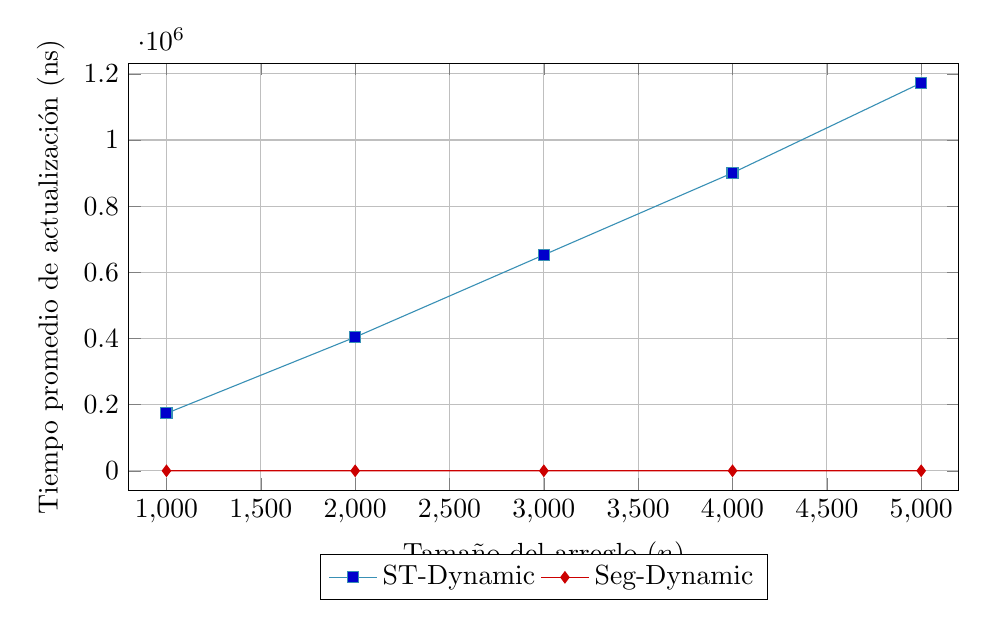
\begin{tikzpicture}
\begin{axis}[
  width=\textwidth,
  height=7cm,
  xlabel={Tamaño del arreglo ($n$)},
  ylabel={Tiempo promedio de actualización (ns)},
  grid=major,
  legend style={at={(0.5,-0.15)},anchor=north,legend columns=2},
  yticklabel style={/pgf/number format/fixed},
  enlargelimits=0.05
]
\addplot+[mark=square*, color=cyan!70!black] coordinates {
(1000,173985.5388888889)
(2000,404226.3077777778)
(3000,652880.1133333333)
(4000,900575.2055555555)
(5000,1172490.0744444444)
};
\addlegendentry{ST-Dynamic}
\addplot+[mark=diamond*, color=red!80!black] coordinates {
(1000,407.8855555555556)
(2000,393.5833333333333)
(3000,426.78777777777776)
(4000,433.6611111111111)
(5000,446.6166666666667)
};
\addlegendentry{Seg-Dynamic}
\end{axis}
\end{tikzpicture}
\caption{Comparación del tiempo promedio de actualización para Sparse Table y Segment Tree dinámicos.}
\end{figure}
